% Created 2019-06-19 Wed 11:05
% Intended LaTeX compiler: pdflatex
\documentclass[11pt]{article}
\usepackage[utf8]{inputenc}
\usepackage[T1]{fontenc}
\usepackage{graphicx}
\usepackage{grffile}
\usepackage{longtable}
\usepackage{wrapfig}
\usepackage{rotating}
\usepackage[normalem]{ulem}
\usepackage{amsmath}
\usepackage{textcomp}
\usepackage{amssymb}
\usepackage{capt-of}
\usepackage{hyperref}
\usepackage{minted}
\usepackage[margin=2cm]{geometry}
\usepackage{enumitem}
\usepackage{svg}
\DeclareMathOperator{\sign}{sign}
\setlength{\parindent}{0cm}
\usepackage{pgfplots}
\pgfplotsset{compat=1.11}
\usetikzlibrary{arrows, decorations.markings}
\usetikzlibrary{3d}
\usetikzlibrary{shapes.geometric,decorations.fractals,shadows}
\date{\today}
\title{}
\hypersetup{
 pdfauthor={},
 pdftitle={},
 pdfkeywords={},
 pdfsubject={},
 pdfcreator={Emacs 26.2 (Org mode 9.1.9)}, 
 pdflang={English}}
\begin{document}


\section{Supervised learning}
\label{sec:org2e4a623}
Method where you train the program by feeding the learning algorithm with a mapping of
inputs to correct outputs.
\subsection{Regression}
\label{sec:org53aa172}
Regression is curve fitting: learn a continuous input \(\to\) output mapping from a set of
examples.
\subsection{Classification}
\label{sec:org436b11d}
Outputs are discrete variables (category labels). Learn a decision boundary that
separates one class from the other. Generally, a confidence is also desired, i.e.,
how sure are we that the input belongs to the chosen category.
\subsection{Training set}
\label{sec:orgcb2c4ad}
The training set is a set of \(m\) \((\vec{X},\, y)\) pairs, where:
\begin{align*}
  \vec{X} \in \mathbb{R}^d & \quad\text{models the input.} \\
  y \in \{0, 1\} & \quad\text{models the output.}
\end{align*}
\subsection{Error function}
\label{sec:orgc44b132}
The loss function for a model \(f: \vec{X} \mapsto y\) parameterized by \(\vec{W}\) applied to a
dataset \(\{ (\vec{X},\, y) \}\) of size \(m\) is:
\[
  L(\vec{W}) = \sum^m_i{ \left(f_{\vec{W}}(\vec{X}_i) - y_i \right)^2 }
\]
\subsection{Perceptron}
\label{sec:org74550ff}
Perceptron is the trivial neural network. The model for a parameter \(\vec{W} = (\text{threshold},\,
   w_1,\, \hdots,\, w_d)\) and inputs of the form \((1,\, x_1,\, \hdots,\, x_d)\) is given by
\[
  f_{\vec{W}}(\vec{X}) = \sign(\vec{W} \vec{X})
\]
Where \(\sign\) is the activation function. \\
If \(x_i\) is evidence for approval, then \(w_i\) should be high. \\
If \(x_i\) is evidence for denial, then \(w_i\) should be low.
\subsubsection{Learning algorithm}
\label{sec:org68a43e9}
The learning algorithm of the Perceptron is quite simple. The learning rate \(\in (0,\,
    1]\) is used to scale each step. the For a training set \(S = \{ \, (\vec{X}_1,\, y_1),\enspace (\vec{X}_2,\,
    y_2),\enspace \hdots \, \}\)
\begin{itemize}[itemsep=0pt]
\item Starting with random weights, then show each sample in sequence repetitively.
\item If the output is correct, do nothing.
\item If the produced output is negative, and the correct output is positive, increase the weights.
\item If the produced output is positive, and the correct output is negative, decrease the weights.
\item The amount to increase/decrease is given by the current sample scaled by the learning rate.
\end{itemize}
\subsection{Error}
\label{sec:org96cd118}
The error function for a model \(f\) in a \textbf{training} sample is
\[ E_{\text{in}}(f) \]
This function is known and calculable. \\

The error function for a model \(f\) in a \textbf{hypothetical} sample is
\[ E_{\text{out}}(f) \]
This function is \textbf{not} known, and only \textbf{approachable}. \\

A good approximation of \(E_{\text{out}}\)(f) is the error in a \textbf{test} (or \textbf{validation})
sample
\[ E_{\text{val}}(f) \]

Given a model \(f\) in a set of \(M\) models, the bound for the probability of the error
deviation surpassing a given \(\epsilon\) is
\[
  \mathbb{P}\left(\big| E_{\text{in}}(f) - E_{\text{ou}t}(f) \big| > \big\epsilon\right) \leq 2Me^{-2N\big\epsilon^2}
\]
Notably, \(E_{\text{in}}(f)\) and \(E_{\text{out}}(f)\) deviates as \(f\) becomes complex.
\subsubsection{Empirical error minimization}
\label{sec:orgc8c3720}
During the learning algorithm, always conserve the weights that produce the lower error. \\
This has a disadvantage: It memorizes the training set.
\subsection{Learning decision trees}
\label{sec:org048ac65}
Each layer in the tree consists of an attribute that splits the data into subsets that
are ideally disjoint. \\
The entropy of the subsets produced is a measure of how disjoint they are. \\

For a set containing \(p\) positive and \(n\) negatives, the entropy is
\[
  H\left(\frac{p}{p+n}, \frac{n}{p+n} \right) = - \frac{p}{p + n} \log\left( \frac{p}{p + n} \right)
                                                - \frac{n}{p + n}\log\left( \frac{n}{p + n} \right)
\]
A given attribute \(A\), with \(k\) distinct values, divides the training set \(S\) into
subsets \(S_1, S_2, \hdots, S_k\). \\
The expected entropy remaining after applying \(A\) is
\[
  EH(A) = \sum_{i = 1}^{k} \left[ \frac{p_i + n_i}{p + n} \cdot H\left( \frac{p_i}{p_i + n_i}, \frac{n_i}{p_i + n_i} \right) \right]
\]
The information gain, i.e. the reduction in entropy for \(A\), is
\[
  I(A) = H\left( \frac{p}{p + n}, \frac{n}{p + n} \right) - EH(A)
\]
\subsection{Capacity}
\label{sec:org9c53397}
The capacity is a measure of when the training error is a good approximation for the
test error.
\begin{figure}[H]
  \centering
  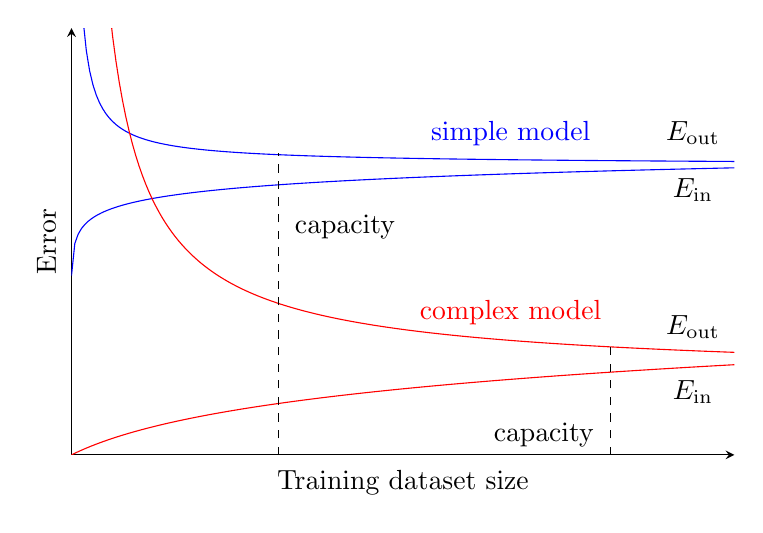
\begin{tikzpicture}
    \begin{axis}[
        axis lines = middle,
        xlabel near ticks,
        ylabel near ticks,
        xlabel     = {Training dataset size},
        ylabel     = {Error},
        xmin       = 0,
        ymin       = 0,
        ymax       = 15,
        height     = 7cm,
        width      = 10cm,
        xtick      = \empty,
        ytick      = \empty,
        black
      ]
      \addplot [
        samples=200,
        domain=0:8,
        blue
      ] {(ln(200*x + 1)/ln(7)) + 6.3};
      \addplot [
        samples=200,
        domain=0.1:8,
        blue
      ] {1/log2(x + 1) + 10};
      \addplot [
        samples=200,
        domain=0:8,
        red
      ] {log2(x + 1)};
      \addplot [
        samples=200,
        domain=0.1:8,
        red
      ] {1/log10(x/2.5 + 1) + 2};

      \draw [black, dashed] (axis cs: 6.5, 0) |- (axis cs: 6.5, 4);
      \draw [black, dashed] (axis cs: 2.5, 0) |- (axis cs: 2.5, 10.6);
      \node [black] at (7.5, 2.2) {$E_{\text{in}}$};
      \node [black] at (7.5, 4.5) {$E_{\text{out}}$};
      \node [black] at (7.5, 9.3) {$E_{\text{in}}$};
      \node [black] at (7.5, 11.3) {$E_{\text{out}}$};
      \node [blue] at (5.3, 11.3) {simple model};
      \node [red] at (5.3, 5) {complex model};
      \node [black] at (3.3, 8) {capacity};
      \node [black] at (5.7, 0.7) {capacity};

    \end{axis}
  \end{tikzpicture}
\end{figure}
\subsection{Bias and variance}
\label{sec:org1c6a278}
\textbf{Bias} is the error due to the fact that the set of functions does not contain the
target function. \\

\textbf{Variance} is the error due to the fact that if we had been using another training set
drawn from the same distribution, we would have obtained another function. \\

\textbf{Regularization} is a method for minimizing the training error, as long as it is still a
good approximation for the test error, trading-off accuracy for simplicity.
\subsection{Single layer neural networks}
\label{sec:org09af160}
Using the sigmoid as the activation function, and the squared-error loss function:
\[
  L(\vec{W}) = \frac{1}{2} \sum_i^m \left( \sigma\left(\vec{W} \vec{X}_i\right) - y_i \right)^2
\]
To find in which direction the weights minimizes \(L\), the gradient is used:
\[
  \nabla L(\vec{W}) = \sum_i^m \Delta \cdot \Psi
\]
Where the delta rule is
\[
  \Delta = \vec{X}_i \cdot \left( \sigma\left(\vec{W}\vec{X}_i\right) - y_i \right)
\]
And the slope of ligistic is
\[
  \Psi = \sigma\left(\vec{W}\vec{X}_i\right) \cdot \left(1 - \sigma\left(\vec{W}\vec{X}_i\right)\right)
\]
\newpage
\subsubsection{Gradient descent algorithm}
\label{sec:org91bc2e9}
The learning rate \(r \in (0,\, 1]\) is used to scale each step.
\begin{enumerate}
\item Starting with random weights.
\item Compute \(\nabla L(\vec{W})\).
\item \(\vec{W} \leftarrow \vec{W} - r \cdot \nabla L(\vec{W}) = \vec{W} - r \cdot \sum\limits_i^m \Delta \Psi\)
\item Repeat steps 2 and 3 until \(\vec{W}\) doesn't change anymore \((10^{-5})\).
\end{enumerate}
After each iteration, \(L(\vec{W})\) should be checked:
\begin{enumerate}
\item If \(L(\vec{W})\) is converging, the learning rate is correct.
\item If \(L(\vec{W})\) is diverging, the learning rate is too large.
\item If \(L(\vec{W})\) is converging slowly, the learning rate too small.
\end{enumerate}
Also, the algorithm needs feature scaling
\[
  x'_i = \frac{x_i - \min(\vec{X})}{\max(\vec{X}) - \min(\vec{X})}
\]
\subsubsection{Stochastic gradient descent}
\label{sec:orgaf49930}
Instead of inspecting the whole dataset to detect the direction which minimize \(L\), a
single random sample is picked on each step.
\begin{enumerate}
\item Randomly shuffle the training set.
\item Starting with random weights.
\item For each sample \((\vec{X_i}, y_i)\): \(\>\vec{W} \leftarrow \vec{W} - r \cdot \Delta \Psi\)
\item Repeat step 3 until \(\vec{W}\) doesn't change anymore \((10^{-5})\).
\end{enumerate}
Convergence is not so obvious. After each bulk of iterations, e.g. 1000, check \(L(\vec{W})\):
\begin{enumerate}
\item If \(L(\vec{W})\) is converging, the learning rate is correct.
\item If \(L(\vec{W})\) is diverging, the learning rate is too large.
\item If \(L(\vec{W})\) is converging slowly, the learning rate too small.
\end{enumerate}
\subsubsection{Mini batches}
\label{sec:org055a479}
While GD uses all samples in each iteration, SGD uses only one. A possible middle
ground is to use a mini batch of samples in each iteration.
\[
  \vec{W} \leftarrow \vec{W} - r \cdot \frac{1}{b} \sum\limits_i^b \Delta \Psi
\]
Where \(b\) is the batch size, tipically \(10\).
\subsubsection{Regularization}
\label{sec:orgf46dbdc}
To prevent large weights, the norm of the weights is added to the loss function:
\[
  L(\vec{W}) = |\vec{W}| + \frac{1}{2} \sum_i^m \left( \sigma\left(\vec{W} \vec{X}_i\right) - y_i \right)^2
\]
\subsubsection{Early stopping (cross validation)}
\label{sec:orgf13c9c6}
Other way to improve is to prevent overfitting:
\begin{enumerate}[itemsep=0pt]
\item Separate the data into training and validation sets.
\item Minimize \(L(\vec{W})\) on the training set, stopping when \(L(\vec{W})\) on the validation set
stops improving.
\end{enumerate}
\subsection{Multi layered neural networks}
\label{sec:org4456326}
This approach introduces one or more hidden layers in the network, each with one or
more neurons. \\
The model for a hidden layer \(h\) is the aggregation of the models of each neuron \(i\) in
the layer.
\[
  y_{h,i} = \sigma \left( \vec{W}_i \, \vec{X}_h \right) \\
\]
The aggregation of the outputs of the layer defines the input for the neurons in the next layer
\[
  X_{h^+} = \left(1,\, y_{h, 1},\, \hdots,\, y_{h, i}\right)
\]
In practice, the layer's weights are aggregated in a matrix, performing the calculation
in a single take. \\
One implication is that the number of neurons in the hidden layers is directly
proportional to the model's complexity.
\subsubsection{Backpropagation}
\label{sec:org57b7614}
\begin{enumerate}
\item Starting with random weights.
\item For each sample, calculate the model, and if the result is incorrect:
\begin{enumerate}
\item Calculate \emph{local gradients} for each neuron. \\
For the neuron \(l\) in the last layer \(k\):
\[
  \delta_{k,l} = \sigma'\left( \vec{W}_l \, \vec{X}_k \right) \cdot (y - y_l)
\]
For the hidden neurons, let \(i^+\) be the attached neuron in the next layer:
\[
  \delta_{h,i} = \sigma'\left( \vec{W}_i \, \vec{X}_h \right) \cdot \left( \delta_{h^+,i^+} \,\cdot\, w_{h^+,i^+} \right)
\]
\item Update the weights with the delta rule. \\
Let \(w_{h,i,j}^+\) be the updated weight, \(w_{h,i,j}\) the current weight, and
\(w_{h,i,j}^-\) the previous weight:
\[
  w_{h,i,j}^+ = w_{h,i,j} + \gamma w_{h,i,j}^- + r \cdot \delta \cdot x_{h,i,j}
\]
Where \(\gamma\) is the momentum, a constant defined to prevent local optima.
\end{enumerate}
\end{enumerate}
\subsection{Support Vector Machines}
\label{sec:orgce0fb4a}
The VC dimension of a model is the higher number of samples for which it can solve \textbf{any}
learning problem. \\
Therefore, the VC dimension is an estimate of the capacity of a model. \\

The VC dimension for a model \(f\) and a training set of size \(n\) is also a bound on the
test error
\[
  L_{\text{test}}(f) \leq L_{\text{train}}(f) + O\left(\sqrt{\frac{\text{VC}(f)}{n}}\right)
\]
To reduce the test error:
\begin{enumerate}[itemsep=0pt]
\item Keep the training error low.
\item Minimize \(\text{VC}(f)\).
\end{enumerate}
By limiting the data to a sphere, we can place a bound on the VC dimension. \\
Let \(d\) be the dimensionality of the data, \(D\) the diameter of the sphere, and
\(\rho\) the margin of the model
\[
  \text{VC}(f) \leq \min\left( d, \left\lceil \frac{D^2}{\rho^2} \right\rceil \right)
\]
Therefore, by maximizing \(\rho\), \(\text{VC}(f)\) becomes \textbf{independent of the dimensionality of
the data}.
\subsubsection{Kernels}
\label{sec:org38da101}
A kernel allows one to map the entries to a higher dimensional feature space, possibly
allowing simpler ways to delimit such entries. \\
One example is the polynomial kernel:
\[
  \left(\vec{x} \cdot \vec{y}\right)^n
\]
\subsection{Neural networks versus SVMs}
\label{sec:orgfdcc25d}
\begin{enumerate}[itemsep=0pt]
\item Linear SVMs are similar to a Perceptron, but with an optimal cost function.
\item If a Kernel is used, then SVMs are comparable to 2-layer neural networks.
\item A 3-layer neural network might correspond to an ensemble of multiple Kernel SVMs.
\end{enumerate}
\subsection{Naive Bayes}
\label{sec:orga6c47ee}
Assuming conditional independence between the input dimensions, the probability of the
target can be approximated using the Bayes theorem:
\[
  P\big(y \>|\> x_1, \hdots, x_d \big) \approx P(y) \cdot \prod_{i}^{d} P\big( x_i \>|\> y \big)
\]
\newpage
\subsection{Ensemble learning}
\label{sec:org947a61d}
Ensemble learning consists in combining several simple models to form a more complex
model.
\begin{description}
\item[{Bagging:}] Each model training with a different dataset
\item[{Boosting:}] Same dataset, but instrumented for each model to mitigate the weakness of
others
\end{description}
\subsection{Boosting}
\label{sec:org102a1da}
Boosting is the technique of combining simple models iteratively to create a complex
model. \\
Each model is intentionally \textbf{biased} to avoid the errors of the previous model. \\

One simple method of boosting is the \textbf{additive boosting}: \\
Considering binary classifiers
\begin{align*}
  & h: \vec{X} \mapsto y \\
  & y \in \{ -1, 1 \}
\end{align*}
The model is defined as
\[
h(\vec{X}) = \sign\big(h_1(\vec{X}) + \hdots + h_n(\vec{X})\big)
\]
\subsubsection{Adaboost}
\label{sec:org63722a9}
The adaptive boosting algorithm is an additive algorithm, with associated importances:
\[
  h(X) = \sign\big(\alpha_1 \cdot h_1(X) + \hdots + \alpha_n \cdot h_n(X)\big)
\]
The adaboost algorithm is \textbf{always based on very simple models}, usually decision
stumps. \\
As a consequence, it \textbf{does not overfit}.
\subsection{Bagging}
\label{sec:orgb57c293}
Boostrap aggregation is the technique of combining models trained in subsets of the
training dataset. \\
The subsets are constructed by uniformly sampling the dataset, and may contain
intersections. \\
\textbf{Small} subsets \textbf{prevent} the base models from \textbf{overfitting}, and therefore bagging
circumvents \textbf{variance} in the data. \\

The models may be combined using many techniques:
\begin{itemize}[itemsep=0pt]
\item Majority voting.
\item Averaging probabilites.
\item Averaging estimates.
\item Etc.
\end{itemize}
In practice, the base models are usually decision trees.
\subsubsection{Random forests}
\label{sec:orgfcf335b}
Random forests exploits randomness in instances and features. \\
Each decision tree is trained with a random subset of \textbf{features} and instances. \\
As a consequence, random forests circumvent overfitting in decision trees.
\subsection{Semi-supervised learning}
\label{sec:orge83a372}
Semi-supervised learning is the method of combining supervised and unsupervised
learning, usually when there are small ammounts of labeled data, and large amounts of
unlabeled data.
\subsubsection{Active learning}
\label{sec:org28ed2ce}
Active learning is a technique to create optimal training sets, by filtering samples
with redundant information. \\

The technique is commonly used in two situations:
\begin{description}[itemsep=0pt]
\item[{Semi-supervised:}] use active learning to obtain a small optimal subset of samples
to label manually.
\item[{Supervised:}] use active learning to balance classes, e.g. for classifying
anomalies, where there are few positive samples.
\end{description}
\vspace{5px}  There are many methods for selecting samples:
\begin{description}
\item[{Uncertainty sampling:}] Select the samples for which the model is least certain
about the correct output.
\item[{Committee:}] Train a comittee of models on the labeled data. Select the unlabeled
samples for which the committee disagrees most.
\item[{Expected model change:}] Select the samples with greater impact on the model.
\item[{Expected error reduction:}] Select the samples with greater impact on the model's
generalization error.
\end{description}
\section{Unsupervised learning}
\label{sec:org24b1b7e}
Unsupervised learning consists to, given only inputs as training, find a pattern:
\begin{itemize}[itemsep=0pt]
\item Clusters
\item Manifolds
\item Embeddings
\item Etc.
\end{itemize}
\subsection{Distance function}
\label{sec:org953bc3f}
Some common distance functions are:
\begin{description}
\item[{Nearest neighbor:}] \(\min({|x - y|}^2)\)
\item[{Furthest neighbor:}] \(\max({|x - y|}^2)\)
\item[{Centroid:}] \({|\mu_i - \mu_j|}^2\)
\end{description}
\subsection{Hierarchical agglomerative clustering}
\label{sec:org44a8e99}
The hierarchical agglomerative clustering technique constructs a dendogram based on a
distance function. \\
Starting with individual clusters, it iteratively merges the closest ones until the
dendogram is complete. Finally, a cut across the dendogram corresponds to a similarity
threshold.
\subsection{K-Means}
\label{sec:orgf698046}
The K-Means algorithm constructs clusters by placing centroids and agglomerating by the
closest centroid. \\
Considering \(k\) clusters, place \(k\) centroids in the space. Update the centroids
iteratively using an expectation-maximization algorithm:
\begin{itemize}[itemsep=0pt]
\item Each cluster is defined by the points that are closest to the correspondent centroid.
\item The centroids are updated with the mean of the points in it's cluster.
\end{itemize}
This technique can be interpreted as optimizing a loss function
\[
  L = \sum_i \left| x_i - \mu_j \right|^2
\]
Different initial centroids may lead to different final losses, motivating different
initialization methods:
\begin{description}[itemsep=0pt]
\item[{Random:}] May choose nearby points
\item[{Distance based:}] Limits the search space, not enough randomness.
\item[{Random and distance based:}] Choose far points randomly.
\end{description}
The choice of \(k\) also impacts the disposition of results:
\begin{description}[itemsep=0pt]
\item[{Small \(k\):}] loose clustering.
\item[{Large \(k\):}] any point is a group itself.
\end{description}
To prevent an overly large \(k\), we must penalize complexity (regularization):
\[
  L = \log \left( \frac{1}{n \cdot d} \cdot \sum_i \left| x_i - \mu_j \right|^2 \right) + k \cdot \frac{\log{n}}{n}
\]
Where \(d\) is the dimensionality of the data, which also plays a fundamental role. With
more dimensions, points tend to get sparse. Therefore, the more dimensions there are,
the more samples one will need.
\subsection{Mixture model}
\label{sec:org5e27150}
The mixture model constructs clusters by assigning probabily distributions and
agglomerating by the most probable distribution. Therefore, it differs from K-Means by
allowing overlaping clusters. \\
As in the K-Means algorithm, the distributions are randomly initialized, and updated
using an expectation-maximization algorithm.
\section{Reinforcement learning}
\label{sec:orgf9737e1}
Method where you train the program by rewarding the learning algorithm positively or
negatively according to the produced results. This method is similar to how we teach
animals.
\pagebreak
\section{Deep learning}
\label{sec:org36a970a}
Deep learning is suitable for problems where the features are not well defined:
\begin{itemize}[itemsep=0pt]
\item Images
\item Text
\item Audio
\end{itemize}
\subsection{Convolutional neural networks}
\label{sec:orgf6fc7e7}
Convolutional neural networks are composed of two sets of layers:
\begin{enumerate}[itemsep=0pt]
\item Alternate layers of:
\begin{description}
\item[{Convolution:}] A mathematical method to identify correlation, extracting features
from the input.
\item[{Pooling:}] A method to reduce dimensionality without loosing information.
\vspace{3pt}
\end{description}
\item A multilayer perceptron, i.e. a neural network.
\end{enumerate}
The convolution step is parameterized by:
\begin{description}[itemsep=0pt]
\item[{Depth:}] the number of filters
\item[{Stride:}] the slide step
\item[{Zero-padding:}] whether to add padding to allow patterns in the borders.
\end{description}
\subsection{Natural language processing}
\label{sec:org2455d6b}
As in convolutional networks, the key technique is how to extract features from the
input. \\
To learn how to represent data, a network composed of two sets of layers is used to
predict the next word in the text:
\begin{enumerate}[itemsep=0pt]
\item The input layer.
\item A multilayer perceptron, i.e. a neural network.
\end{enumerate}
For training, each word in the vocabulary is initally modeled as a random vector. \\

By allowing training of the input layer itself, the network \textbf{learns} how to
significantly model the inputs for the given dataset. Therefore, after training, the
network has not only produced the prediction model, but also a feature model in the
first layer. This feature model can be used as input layer for any other network,
including networks with other targets.
\subsection{Unsupervised feature learning}
\label{sec:org7e4f9c2}
\subsubsection{Autoencoder}
\label{sec:orgaac1689}
The autoencoder is a neural network with one hidden layer that implements a lossy
compression machine. By compressing and decompressing the input, it removes irrelevant
data due to the loss. Such network can be trained as it was supervised, as the
expected output is the input itself. \\

Because the hidden layer has a smaller dimension than the input, it can be used with
the input layer as a feature model that reduces the dimensionality.
\subsection{Generative adversarial networks}
\label{sec:org7e90ab1}
Generative adversarial networks aim to train a generative network, using an
discriminative network. \\
Both networks compete in a zero-sum game, that converges when both players don't
change their output given the oponent's output.
\begin{center}
\includesvg[width=200px]{images/gan}
\end{center}
The error function for the generator is whether the discriminator missed.
\end{document}
